\section{Data Preparation}
We choose online textual news as our corpus because it is available in large volumes. 
And more importantly it contains title field and body field. We assume title
field is the outline of the subject and the body field elaborates the details. 
Based on this assumption, the abstraction nouns are
likely to be found in news titles and the action instances should 
follow accordingly in the news bodies.

The news corpus we use is provided by Bing news. It includes around
5 million unique news entries with URLs pointing to the original 
online versions. 

\begin{figure}[h!]
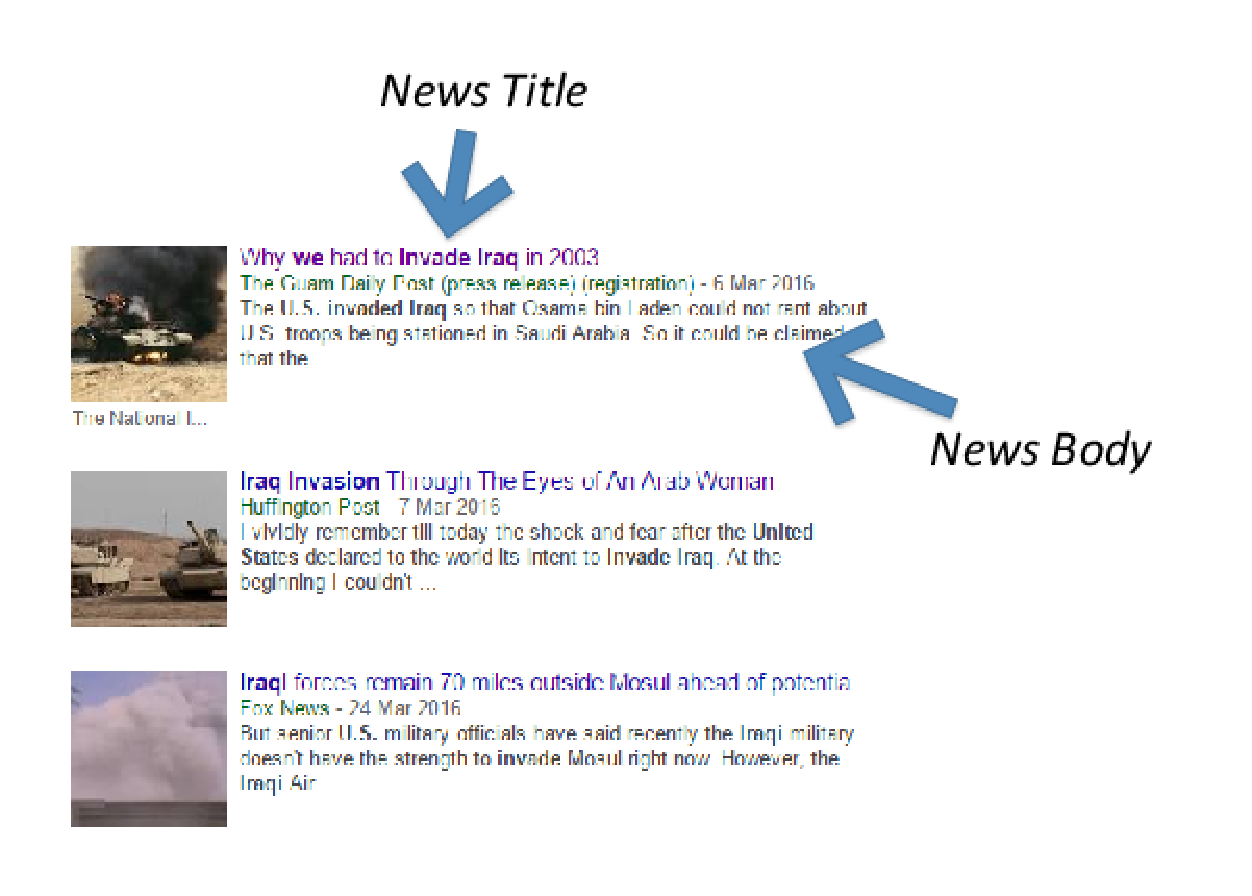
\includegraphics[width=\linewidth]{img/ac3}
\caption{News}
\label{fig:news}
\end{figure}


In order to extract action instances from news body, we first need to 
parse the news body into Penn trees and Postag each word in both
the titles and bodies. Next we manually chose around 100 action concepts
from previous work by \cite{gong2015representing}. Finally we need to construct a noun
concept dictionary as our abstraction inventory. This can be done in 
multiple ways, for instance by using the lexical information provided by
wordnet \cite{wn} or generating such nouns from Probase \cite{wu2012probase}. 

Specifically, in wordnet there is a field called lexical info for each token,
such as ``noun.act'', ``noun.state''. We can use these information to generate an
initial noun pool. In this stage Probase could be used in two ways, firstly it
can also be used as a pool generator. We can build the noun pool by manually designing
a small set of terms that has desired nouns as hyponyms, such terms include ``activity'',
``process'', ``event'' etc. Secondly probase can also be used as a filter. We check how 
many instances a noun could have and use it as a measurement to decide whether it 
is abstract noun or concrete instances. Probase also provides the likelihood of 
the hypernym-hyponym relations which we could use too. Wikitionary \cite{wiktionary} is an online 
dictionary, we found a list of top 10000 popular English word there, hoping to 
solve the problem that some words in Wordnet or Probase are too obsolete.
Overall we have 4 different methods to generate the dictionary:
\begin{enumerate}
\item Use top 10000 English word as initial pool and filter by Probase
\item Use Wordnet noun iterator, combined with lexical info to build the initial pool and filter by Probase
\item Use Probase to generate the initial pool and filter by Probase
\item Use Wordnet noun iterator, combined with lexical info, no filtering
\end{enumerate}

